\documentclass[12pt]{exam}
%\documentclass[12pt]{article}
\usepackage[letterpaper, margin=0.75in]{geometry}
\usepackage{graphicx}
\usepackage{enumitem}
\usepackage{booktabs}
\usepackage{amsmath}
\usepackage{tabularx}
\usepackage{color}

\begin{document}
\footer{}{Page \thepage\ of \numpages}{}

\begin{flushright}
\makebox[0.5\textwidth]{\large Name:\enspace\hrulefill}
\vspace{0.2in}
\end{flushright}

\begin{center}

\includegraphics[width=10cm]{../images/logo.png}
\end{center}

\begin{center}
\noindent{\LARGE Conceptual Physics \\ Class 13 Questions \\ May 4th, 2018 \\}
\end{center}
\vspace{0.5in}

\vspace{0.2in}

The following might be useful for today's class questions:
\begin{center}
\noindent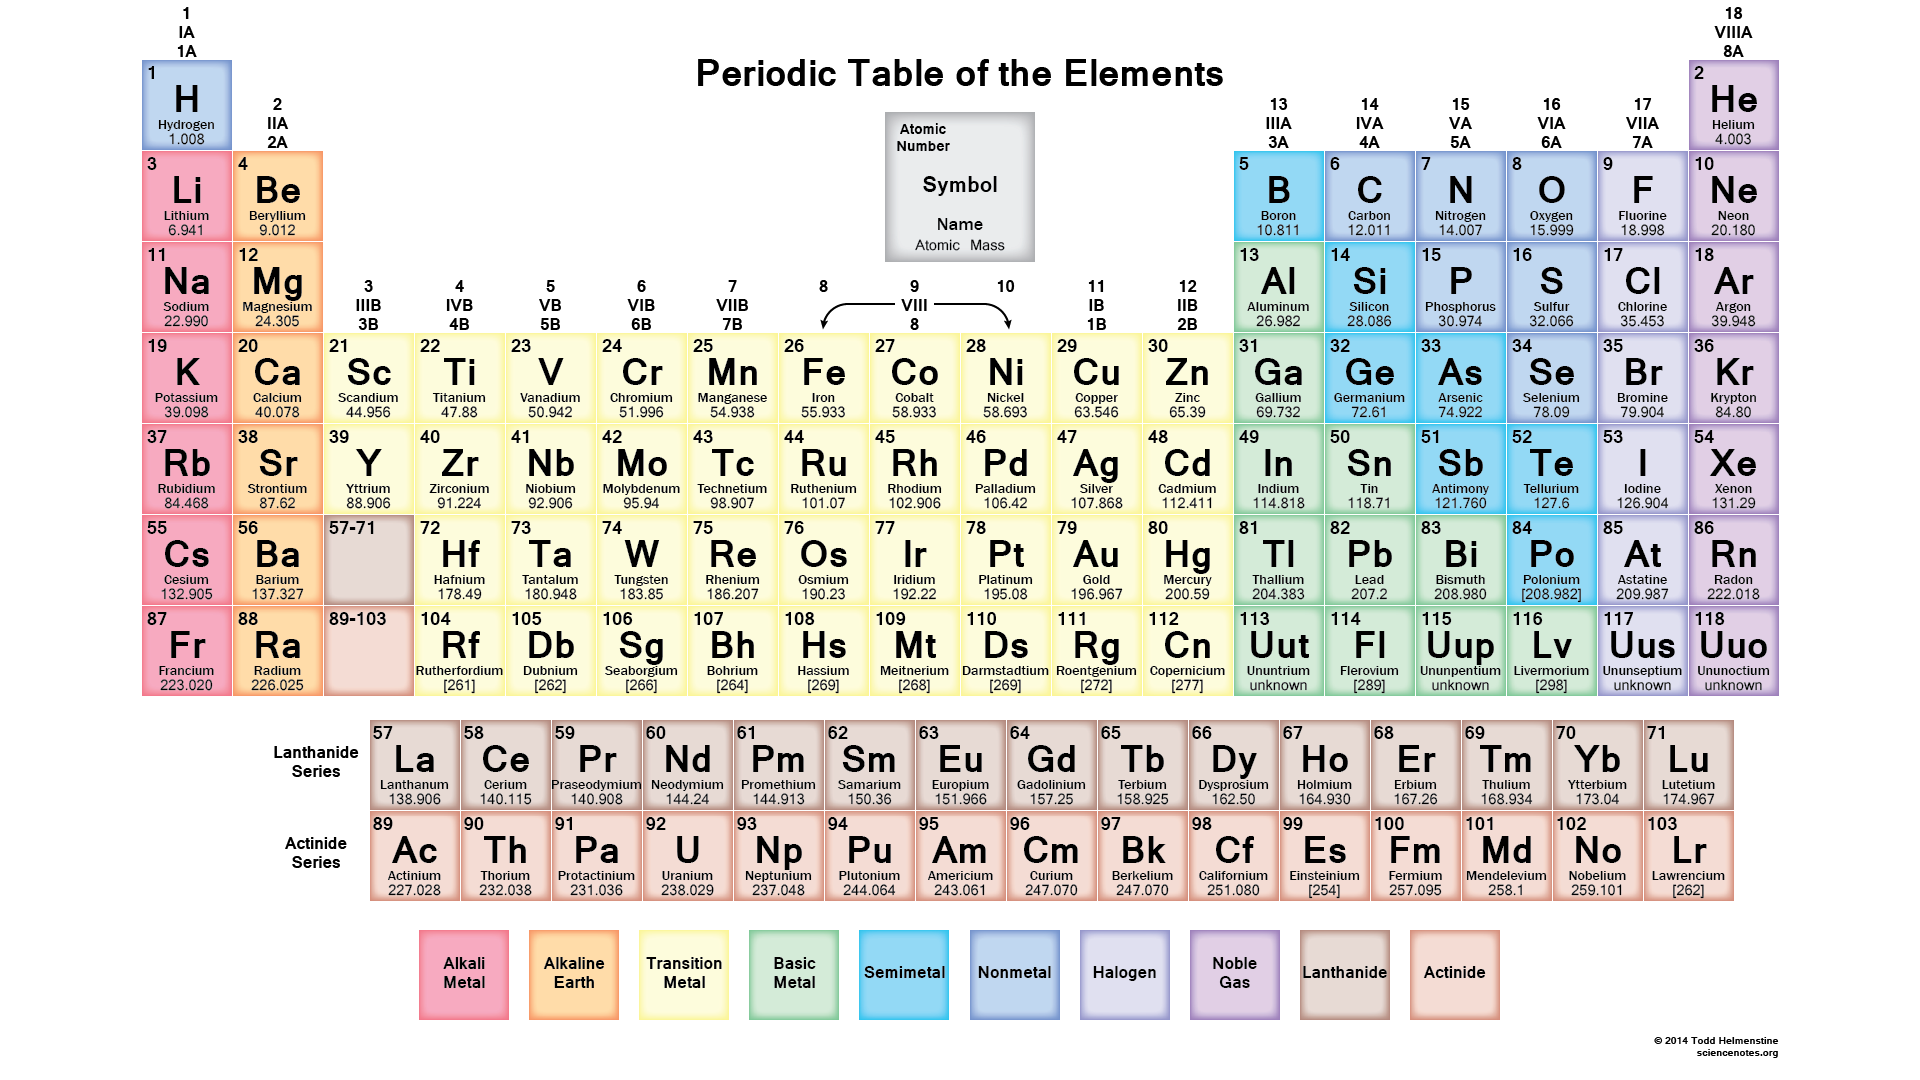
\includegraphics[width=\textwidth]{../images/periodicTable.png}
\end{center}


\clearpage

\noindent\textbf{\Large Part 1: Probability}
\begin{questions}
	\question You have a jar with 73 red balls, and 27 blue balls. You randomly draw a ball from this jar. What is:
		\begin{parts}
			\part The percent chance that you will draw a red ball?
				\vspace{0.3in}
			\part The percent chance that you will draw a blue ball?
				\vspace{0.3in}
			\part The probability that you will draw a red ball?
				\vspace{0.3in}
			\part The probability that you will draw a blue ball?
				\vspace{0.3in}
			\part The probability of drawing a red or blue ball?	
				\vspace{0.3in}
		\end{parts}
		
	\question Give an example of 2 statistically \textit{independent} events.
		\vspace{0.5in}
		
	\question Give an example of 2 statistically \textit{dependent} events.
		\vspace{0.5in}
		
	\question You toss a coin in the air 3 times. What is the probability that:
		\begin{parts}
			\part It will land heads all 3 times?
				\vspace{0.5in}
			\part It will land heads twice (and only twice)?
				\vspace{0.5in}
			\part It will land heads 2 or 3 times?
				\vspace{0.5in}
			\part It will land tails 2 or 3 times?
				\vspace{0.3in}
		\end{parts}
		
	
	\clearpage
\question You are tossing a fair coin, which has a 1/2 probability of landing heads and a 1/2 probability of landing tails. If you toss the coin in the air 300 times, how many times \textbf{on average} would you expect it to land:
	\begin{parts}
		\part Heads:
			\vspace{0.5in}
		\part Tails:
			\vspace{0.5in}
	\end{parts}
\question You are tossing a trick coin, which has a 2/3 probability of landing heads, and a 1/3 probability of landing tails. If you toss the coin 300 times, hoe many times \textbf{on average}	 would you expect it to land:
	\begin{parts}
		\part Heads:
			\vspace{0.5in}
		\part Tails:
			\vspace{0.5in}
	\end{parts}
	
\question Based on your answers to the two previous questions, how could you tell if a coin was fair (without any special equipment or knowledge of how coins can be biased)?
	\vspace{1in}
	
	\question There are 52 cards in a deck. You are dealt 2 cards (without refilling the deck). What is the probability that you will have both the ace of spades and the ace of diamonds?
		\vspace{1in}
	
	\question Why isn't it valid to define randomness by saying that randomness is when all outcomes are equally likely?
		
	
	From \textit{Light and Matter}, Chapter 33 Discussion Question B
	\vspace{0.5in}
	
	\clearpage
\question Suppose you have two identical loaded four-sided dice, with P(4) = 1/2, and P(1) = P(2) = P(3) = 1/6. 
\begin{parts}	
	\part If you rolled one die many times, what is the average value you would roll?
		\vspace{1in}
	\part If you rolled both dice there are 16 possible rolls you could get. What is the probability of each?
		\vspace{1in}
	\part If you add up the values of your two rolls, you could get between 2 and 8. What is the probability of each possible sum?
		\vspace{1in}
	\part What is the average sum you would get if you rolled both dice many times?
		\vspace{1in}
\end{parts}

\question Does the number of radioactive nuclei in a sample decrease to exactly half its original value in one half-life? Explain in terms of the statistical nature of radioactive decay.
	\vspace{1in}
	
	\question Describe the following kinds of radioactive decay;
		\begin{parts}
			\part Alpha decay:
				\vspace{0.3in}
				
			\part Beta decay:
				\vspace{0.3in}
				
			\part Gamma decay:
				\vspace{0.3in}
		\end{parts}
		
	\question You have a block of radioactive material, and measure the number of initial decays to be 128 million. If it has a half-life of 4 hours, what do you expect its radioactivity level to be after:
		\begin{parts}
			\part 4 hours?
				\vspace{0.3in}
			\part 8 hours?
				\vspace{0.3in}
			\part 16 hours?
				\vspace{0.3in}
		\end{parts}
		
	\question Does the number of radioactive nuclei in a sample decrease to exactly half its original value in one half-life? Explain in terms of the statistical
nature of radioactive decay.
	\vspace{0.5in}
		
	\question What distinguishes between:
		\begin{parts}
			\item Different kinds of elements?
				\vspace{0.3in}
			\item Different isotopes within an element?
				\vspace{0.3in}
		\end{parts}
		
	\question Physicists thought for a long time that bismuth-209 was the
heaviest stable isotope. (Very heavy elements decay by alpha emission because of the strong electrical repulsion of all their protons.)
However, a 2003 paper by Marcillac et al. describes an experiment
in which bismuth-209 lost its claim to fame — it actually undergoes
alpha decay with a half-life of $2\times 10^{19}$ years.
	\begin{parts}
		\part After the alpha particle is emitted (two protons and two neutrons), what is the isotope left over?
			\vspace{0.5in}
		\part Compare the half-life to the age of the universe, which is about
14 billion years.
			\vspace{0.5in}
	\end{parts}
	
	\question What is the source of energy emitted in radioactive decay? (Hint: think about conservation laws from before)
	\vspace{0.3in}
	
	\clearpage
	\noindent\textbf{\Large Part 2: Quantum Mechanics}
	
	\question What is the Heisenberg uncertainty principle?
		\vspace{0.5in}
		
	\question What is the concept of \textit{wave-particle duality}?
		\vspace{0.5in}
		
	\question How would the wavelength of an object change if:
		\begin{parts}
			\part Its mass increased?
				\vspace{0.3in}
			\part Its velocity decreased?
				\vspace{0.3in}
		\end{parts}
		
	\question Three particles of equal mass are traveling in the same direction. The waves of
the three particles are as shown.
	\begin{center}
		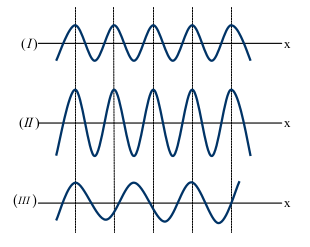
\includegraphics[width=3in]{../images/deBroglie.png}
	\end{center}
	Rank the speeds of the particles ( I ), ( II ) and ( III ) by circling one of these four possibilities.
\begin{choices}
	\choice $v_{II} > v_I > v_{III}$
	\choice $v_{II} > v_{III} > v_I$
	\choice $v_{I} = v_{II} > v_{III}$
	\choice $v_{II} > v_I = v_{III}$
\end{choices}

	\question According to the uncertainty principle, the more we know about an electron's position,
the less we know about its
\begin{choices}
	\choice speed.
	\choice momentum.
	\choice kinetic energy.
	\choice all of these.
\end{choices}

	\question A metal surface is struck with light of wavelength 400nm, releasing a stream of electrons. If the 400nm light is replace by a 300nm light with the same number of photons incident on the metal per second, what will happen?
\begin{choices}
\choice More electrons are emitted in a given time interval
\choice Fewer electrons are emitted in a given time interval
\choice Emitted electrons are more energetic
\choice Emitted electrons are less energetic
\choice None of the above
\end{choices}

\question A metal surface is struck with light of wavelength 400nm, releasing a stream of electrons. If the light intensity increases without changing the wavelength, what will happen?
\begin{choices}
\choice More electrons are emitted in a given time interval
\choice Fewer electrons are emitted in a given time interval
\choice Emitted electrons are more energetic
\choice Emitted electrons are less energetic
\choice None of the above
\end{choices}
	
	\question Why do we not notice quantum effects in our day-to-day lives?	
		\vspace{0.5in}	
	
\end{questions}

\end{document}
